\section{Dipôle magnétique}
\subsection{Définition et ordre de grandeur}

On considère une spire de courant plane présentée à la Figure~\ref{fig:moment_dipolaire_magnetique_spire_plane}. On définit le moment dipolaire magnétique, d'unité $\si{\ampere\metre\squared}$ par
\begin{equation}
    \boxed{
        \vec{m}\coloneqq iS\vec{N}.
    }
\end{equation}
Pour une bobine plate avec 10000 spires, on a $m=niS\approx1\si{\ampere\metre\squared}$.

\begin{figure}
    \centering
    \tikzsetnextfilename{moment_dipolaire_magnetique_spire_plane}
    \begin{tikzpicture}[scale=1]  
        \draw[pattern=north east lines] (0,0) ellipse (2 and 0.5);
        \draw[text=blue,draw=blue,-latex] (0,0)--++(0,1) node [above] {$\vec{N}$};
        \node at (1,0.75) {$S$};
        \node at (0,-0.5) {>};
        \node at (0,-0.75) {$i$};
    \end{tikzpicture}
    \caption{Moment dipolaire magnétique d'une spire de courant plane.}
    \label{fig:moment_dipolaire_magnetique_spire_plane}
\end{figure}

On considère maintenant un électron autour dans un atome à la Figure~\ref{fig:moment_magnetique_orbital}. Par un raisonnement équivalent, on a $i=-e/T$ avec $T$ la période de révolution de l'électron autour du noyau. Alors 
\begin{equation}
    \vec{m}=iS\vec{u}_z=-\frac{e}{T}\pi r^{2}\vec{u}_z.
\end{equation}
Le moment cinétique de l'électron est 
\begin{equation}
    \vec{L}_O=r\vec{u}_r\wedge m\vec{v}=mrv\vec{u}_z,
\end{equation}
d'où
\begin{equation}
    \boxed{
        \vec{m}=\gamma\vec{L}_O,
    }
\end{equation}
avec $\gamma=-e/(2m)$ le rapport gyromagnétique. À l'échelle atomique, on a $\left\lVert\vec{L}_O\right\rVert\approx\hbar\approx10^{-34}\si{\joule\second}$. Alors $\left\lVert\vec{m}\right\rVert\sim10^{-23}\si{\ampere\metre\squared}$.

\begin{figure}
    \centering
    \tikzsetnextfilename{moment_magnetique_orbital}
    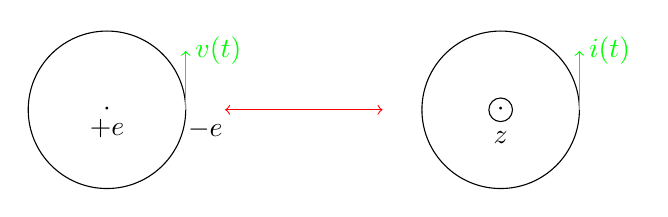
\begin{tikzpicture}[scale=1]
        \draw (5,0) circle (1);
        \node at (5,0) {$\cdot$};
        \draw (5,0) circle (0.15);
        \node at (5,-0.15) [below]{$z$};
        \draw[draw=green, text=green,->] (6,0)--++(0,0.75) node [right] {$i(t)$};
        
        \draw (0,0) circle (1);
        \node at (0,0) {$\cdot$};
        \node at (0,0) [below] {$+e$};
        \draw[draw=green, text=green,->] (1,0)--++(0,0.75) node [right] {$v(t)$};
        \node at (1.25,-0.25) {$-e$};

        \draw[<->,draw=red] (1.5,0)--++(2,0);
    \end{tikzpicture}
    \caption{Moment magnétique orbital d'un électron dans un atome.}    
    \label{fig:moment_magnetique_orbital}
\end{figure}

Au niveau de la terre, le moment magnétique est de l'ordre de $6.10^{2}\si{\ampere\metre\squared}$ (déduit des mesures de $\vec{B}_{\mathrm{terre}}$).

\subsection{Champ magnétique créé par un dipôle magnétique dans l'approximation dipolaire}
\subsubsection{Analyse des symétries}

On fait l'hypothèse que l'on a une spire circulaire de rayon $a$, et on se place en coordonnées cylindriques, l'axe $\vec{u}_z$ passant au centre de la spire, perpendiculairement à celle-ci. On note $\alpha$ l'angle entre l'altitude $z$ du point projeté de $M$ sur l'axe $(Oz)$ et la spire. Alors il y a une symétrie de révolution par rapport à l'axe $(Oz)$, et tout plan contenant $(Oz)$ est un plan d'antisymétrie, on en déduit donc que
\begin{equation}
    \vec{B}(M)=\begin{pmatrix}
        B_{r}(r,\theta)\\ B_{\theta}(r,\theta)\\0
    \end{pmatrix}.
\end{equation}

\subsubsection{Champ dans l'approximation dipolaire}

Donnée: sur l'axe $(Oz)$, on a $\vec{B}_{\mathrm{axe}}(M)=\frac{\mu_0i}{2a}\sin^{3}(\alpha)\vec{u}_z$. On note que $\sin(\alpha)=a/(a^{2}+z^{2})^{-1/2}$, et dans l'hypothèse de l'approche dipolaire, c'est-à-dire $\left\lvert z\right\rvert\gg a$, alors
\begin{equation}
    \vec{B}_{\mathrm{axe}}(z)\approx\frac{\mu_0i}{2a}\frac{a^{3}}{z^{3}}\vec{u}_z=\frac{\mu_0ia^{2}}{2z^{3}}\vec{u}_z=\frac{\mu_0 m}{2\pi z^{3}}\vec{u}_z.
\end{equation}
On admet que cette forme s'adapte autre part que sur l'axe: dans l'approximation dipolaire, on a 
\begin{equation}
    \boxed{
    \vec{B}(M)=\frac{\mu_0 m}{4\pi r^{3}}\begin{pmatrix}
        2\cos\theta\\\sin\theta\\0
    \end{pmatrix}
    .}
\end{equation}
Ainsi, par rapport à la formulation pour le champ électrostatique, il suffit de remplacer $\vec{p}$ par $\vec{m}$, $1/\varepsilon_0$ par $\mu_0$ et $\vec{E}$ par $\vec{B}$.

\subsubsection{Allure des lignes de champ}
Dans l'approximation dipolaire, il y a les mêmes lignes de champ que $\vec{E}$. Mais près de la source, c'est très différent (voir le chapitre sur la magnétostatique).

\subsection{Actions mécaniques subies par un dipôle magnétique plongé dans \texorpdfstring{$\vec{B}^{\mathrm{ext}}$}{B}}
\subsubsection{Champ extérieur uniforme}
On a
\begin{equation}
    \vec{F}_{\mathrm{lor}}=\oint i\vec{\d l}\wedge\vec{B}^{\mathrm{ext}}=i\left[\oint\vec{\d l}\right]\wedge\vec{B}^{\mathrm{ext}},
\end{equation}
donc pour un champ magnétique uniforme, on a $\vec{F}_{\mathrm{lor}}=\vec{0}$.

On peut aussi montrer que le couple de rappel est
\begin{equation}
    \boxed{
        \vec{M}_O=\vec{m}\wedge\vec{B}^{\mathrm{ext}},
    }
\end{equation}
il y a donc un alignement de $\vec{m}$ sur $\vec{B}^{\mathrm{ext}}$.

\subsubsection{Champ non uniforme}
On admet que l'on a 
\begin{equation}
    \boxed{
        \left\lbrace
    \begin{aligned}
        \vec{F}_{\mathrm{lor}}&=\left(\vec{m}\cdot\vec{\grad}\right)\vec{B}^{\mathrm{ext}},\\
        \vec{M}_O&=\vec{m}\wedge\vec{B}^{\mathrm{ext}}.
    \end{aligned}
    \right.}
\end{equation}

Il y a donc un alignement avec le champ magnétique extérieur, et il y a una attraction vers les zones de plus fort champ.

\subsubsection{Énergie potentielle d'interaction}

On retrouve le même résultat formel
\begin{equation}
    \boxed{
        E_p^{\mathrm{ext}}=-\vec{m}\cdot\vec{B}^{\mathrm{ext}},
    }
\end{equation}
et les mêmes discontinuités sur les équilibres stables et instables.